\documentclass[xcolor=pdftex,romanian,colorlinks]{beamer}


 \usetheme{Median}
%% General document %%%%%%%%%%%%%%%%%%%%%%%%%%%%%%%%%%

\usepackage[romanian]{babel}

\setbeamertemplate{footline}[frame number]
\input{beamercolor}
\uselanguage{romanian}
\languagepath{romanian}

\deftranslation[to=romanian]{Proof}{Demonstra\c tie}
\deftranslation[to=romanian]{Example}{Exemplu}
\deftranslation[to=romanian]{Theorem}{Teorem\u a}
\deftranslation[to=romanian]{Solution}{Solu\c tie}
\deftranslation[to=romanian]{Lemma}{Lem\u a}
\deftranslation[to=romanian]{Definition}{Defini\c tie}

\usepackage{alltt}
\usepackage{xcolor}
\usepackage{float}
\usepackage{graphicx,wrapfig}
\usepackage{multirow}
\usepackage{tabularx,colortbl}
\usepackage{listings}  
\usepackage{multicol}  
\usepackage{hyperref}  
\usepackage{tikz}
 
\newcommand{\intens}[1] {{\color{DeepSkyBlue3} #1}}
\newcommand{\myalert}[1] {{\color{MedianOrange} #1}}

\usepackage{../tslides}
\usepackage{comment}

\lstset{language=Haskell}
\lstset{escapeinside={(*@}{@*)}}
\newcommand{\li}[1]{\lstinline$#1$}
\newcommand{\ra}{\rightarrow}
\newcommand{\sra}{\stackrel{*}{\rightarrow}}
 
\begin{document}
\title{\\Curs 6}
\author{Fundamentele Limbajelor de Programare} 
\date{2020-2021} 

\frame{\titlepage} 

 

%\frame{\frametitle{Cuprins}\tableofcontents} 

\begin{frame}{$\lambda$-calcul}

\begin{itemize}
\item În 1929-1932 Church a propus 
$\lambda$-calculul ca sistem formal pentru logica matematică.
În 1935 a argumentat că orice funcție calculabilă peste numere naturale poate
fi calculată in $\lambda$-calcul.

\item În 1935, independent de Church, Turing a dezvoltat mecanismul de calcul
numit astăzi Mașina Turing. 
În 1936 și el a argumentat câ orice funcție calculabilă peste numere naturale poate
fi calculată de o mașină Turing.
De asemenea, a arătat echivalența celor două modele de calcul.
Această echivalență a constituit o indicație puternică asupra "universalității" 
celor două modele, conducând la ceea ce numim astăzi "Teza Church-Turing".
\end{itemize}
\end{frame}

\begin{frame}{Referin\ts e}

\begin{itemize}
\item Benjamin C. Pierce, Types and Programming Languages, The MIT Press 2002
\bigskip
 
\item J.R. Hindley, J.P. Seldin, Lambda-Calculus and Combinators, an Introduction, Cambridge University Press, 2008
\bigskip

\item R. Nederpelt, H. Geuvers, Type Theory and Formal Proof, an Introduction, Cambridge University Press 2014

\end{itemize}
\end{frame}

\begin{frame}[fragile]{ $\lambda$-calcul: sintaxa}

\begin{block}{Lambda Calcul - sintaxă}
\begin{center}
 \begin{tabular}{lll}
$t=$ &  $x$ &  (variabilă) \\
 & $\mid \lambda x.\, t$ & (abstractizare)\\
  & $\mid t\,\, t$ & (aplicare)
\end{tabular}
\end{center}
\end{block}

\pause

\begin{block}{$\lambda$-termeni}

Fie $Var=\{x,y,z,\ldots\}$ o mul\ts ime infinit\u a de variabile.

Mul\ts imea  $\lambda$-termenilor $\Lambda T$ este definit\u a inductiv astfel:
\begin{center}
\begin{itemize}
\item[][Variabil\u a] $Var\subseteq \Lambda T$
\item[][Aplicare] dac\u a $t_1$, $t_2\in \Lambda T$ atunci 
$(t_1t_2)\in \Lambda T$
\item[][Abstractizare] dac\u a $x\in Var$ \sh i $t\in \Lambda T$ atunci
$(\lambda x.t)\in \Lambda T$
\end{itemize} 
\end{center}
\end{block}
\end{frame}




\begin{frame}[fragile]{ Lambda termeni }

\begin{block}{$\lambda$-termeni: exemple}
\begin{itemize}
\item $x$, $y$, $z$

\item  $(xy)$, $(yx)$, $(x(yx))$ 

\item $(\lambda x.x)$, $(\lambda x.(xy))$, $(\lambda z.(xy))$,
$(\lambda x.(\lambda z.(xy)))$ 
 

\item $((\lambda x. x)y)$, $((\lambda x.(xz))y)$, $((\lambda x. x)(\lambda y.y))$
\end{itemize}
\end{block}

\pause

Conven\ts ii:

\begin{itemize}
\item se elimin\u a parantezele exterioare
\item aplicarea este asociativ\u a la st\^{\i}nga: $t_1t_2t_3$ este $(t_1t_2)t_3$
\item corpul abstractiz\u arii este extins la dreapta: $\lambda x.t_1t_2$ este $\lambda x.(t_1t_2)$ (nu $(\lambda x.t_1)t_2$)
\item scriem $\lambda xyz.t$ \^{\i}n loc de $\lambda x.\lambda y.\lambda z.t$
\end{itemize}
\end{frame}

\begin{frame}[fragile]{ Lambda termeni / Funcții anonime}

\begin{block}{$\lambda$-termeni: exemple}
\begin{itemize}
\item $x$, $y$, $z$

\item  $(xy)$, $(yx)$, $(x(yx))$ 

\item $(\lambda x.x)$, $(\lambda x.(xy))$, $(\lambda z.(xy))$,
$(\lambda x.(\lambda z.(xy)))$ 
 

\item $((\lambda x. x)y)$, $((\lambda x.(xz))y)$, $((\lambda x. x)(\lambda y.y))$
\end{itemize}
\end{block}



\begin{block}{$\lambda$-termeni/ func\ts ii anonime în Haskell}
 În Haskell, \structure{\textbackslash} e folosit în locul simbolului \structure{$\lambda$} și
 \structure{\lstinline{->}} în locul punctului.

\begin{tabular}{c@{ este  }c}
$\lambda x. x * x$ & \texttt{\textbackslash x -> x * x}
\\
$\lambda x. x > 0$ & \texttt{\textbackslash x -> x > 0}
\end{tabular}
\end{block}
\end{frame}



\begin{frame}[fragile]{ Variabile libere \sh i legate}

\begin{block}{Apari\ts ii libere \sh i legate}
Pentru un termen $\lambda x.t$ spunem c\u a:
\begin{itemize}
\item apari\ts iile variabilei $x$ \^{\i}n $t$ sunt  legate ({\it bound})
\item $\lambda x$ este leg\u atura ({\it binder}), iar $t$ este domeniul ({\it scope}) leg\u arii
\item o apari\ts ie a unei variabile este liber\u a ({\it free}) dac\u a apare \^{\i}ntr-o pozi\ts ie \^{\i}n care nu e legat\u a.
\end{itemize}

Un termen f\u ar\u a variable libere se nume\sh te \^{\i}nchis ({\it closed}). 
\end{block}

Exemplu:
\begin{itemize}
\item $\lambda x. x$ este un termen \^{\i}nchis
\item $\lambda x. xy$ nu este termen \^{\i}nchis, $x$ este legat\u a, $y$ este liber\u a
\item \^{\i}n termenul $x (\lambda x. xy)$ prima apari\ts ie a lui $x$ este liber\u a, a doua este legat\u a. 
\end{itemize}
\end{frame}

\begin{frame}[fragile]{ Variabile libere}


\begin{block}{Mul\ts imea variabilelor libere $FV(t)$}
Pentru un $\lambda$-termen $t$ mul\ts imea variabilelor libere este definit\u a astfel:
\begin{itemize}
\item[][Variabil\u a] $FV(x)={x}$
\item[][Aplicare] $FV(t_1 t_2) = FV(t_1)\cup FV(t_2)$
\item[][Abstractizare] $FV(\lambda x.t)=FV(t)\setminus \{x\}$
\end{itemize}
\end{block}

Exemplu:

\begin{tabular}{ll}
$FV(\lambda x. xy) =$ & $FV (x y) \setminus \{x\}$ \\
            & ($FV(x)\cup FV(y))\setminus \{x\}$\\
            & $(\{x\}\cup \{y\}) \setminus \{x\}$\\
            & $\{y\}$
\end{tabular}
\pause

\begin{tabular}{ll}
$FV(x\lambda x. xy) =$ & \pause $\{x, y\}$
\end{tabular}
\end{frame}

\begin{frame}[fragile]{ Substitu\ts ii}
Fie $t$ un  $\lambda$-termen $x\in Var$. 

\begin{block}{Defini\ts ie intuitiv\u a}
Pentru un $\lambda$-termen $u$ vom nota prin $[u/x]t$ rezultatul \^{\i}nlocuirii tuturor apari\ts iilor libere ale  lui $x$ cu $u$ \^{\i}n $t$.
\end{block}


Exemple:
Dac\u a $x,y,z$ sunt variabile distincte atunci
\begin{itemize}
\item $[y/x]\lambda z. x=\lambda z. y$ 
 
\item $[(\lambda z.zw)/x](\lambda y.x)= \lambda y. \lambda z. zw$

\end{itemize}
\end{frame}


\begin{frame}[fragile]{ Substitu\ts ii}
\vspace*{0.3cm}

\begin{block}{Definirea substitu\ts iei}
 Rezultatul substituirii lui $x$ cu $u$ \^{\i}n $t$ este definit astfel:

\begin{itemize}
\item[][Variabil\u a] $[u/x]x = u$
\item[][Variabil\u a] $[u/x]y= y$ dac\u a $x\neq y$
\item[][Aplicare] $[u/x](t_1t_2)= [u/x]t_1[u/x]t_2$
\item[][Abstractizare] $[u/x]\lambda y.t=\lambda y. [u/x]t $ unde\\
\hspace*{3cm} $y\neq x$ \sh i $y\not\in FV(u)$
\end{itemize}
\end{block}
\end{frame}

\begin{frame}[fragile]{ Substitu\ts ii}

Exemple:
Dac\u a $x,y,z$ sunt variabile distincte atunci
\begin{itemize}
\item $[y/x]\lambda z. x=\lambda z. y$ 
 \medskip
 
\item  Cine este $[y/x] \lambda y.x$ ?\pause

Dac\u a  folosim defini\ts ia intuitiv\u a ob\ts inem 

$[y/x] \lambda y.x = \lambda y. y$ ceea ce este gre\sh it!\pause


\medskip
Cum proced\u am pentru a repara gre\sh eala? Observ\u am c\u a $\lambda y.x$ desemneaza o func\ts ie constant\u a, aceea\sh i func\ts ie put\^{a}nd fi reprezentat\u a  prin $\lambda z.x$. Aplicarea corect\u a a substitu\ts iei este:

   $[y/x] \lambda y.x=[y/x] \lambda z.x=\lambda z.y$
   
   \pause\medskip
   
   
 {\it Avem libertatea de a redenumi variabilele legate!}
\end{itemize}
\end{frame}


\begin{frame}[fragile]{$\alpha$-conversie ($\alpha$-echivalen\ts \u a)}
\begin{block}{$\alpha$-conversia $=_\alpha$ }
\begin{itemize}
\item[][Reflexivitate] $t=_\alpha t$
\item[][Simetrie]   $t_1=_\alpha t_2$ implic\u a $t_2=_\alpha t_1$
\item[][Tranzitivitate] $t_1=_\alpha t_2$ \sh i $t_2=_\alpha t_3$ implic\u a $t_1=_\alpha t_3$
\item[][Redenumire] $\lambda x.t =_\alpha \lambda y. [y/x]t$ dac\u a $y\not\in FV(t)$
\item[][Compatibilitate]  $t_1=_\alpha t_2$ implic\u a \\
 \hspace*{3cm} $tt_1=_\alpha tt_2$, $t_1t=_\alpha t_2t$ \sh i 
$\lambda x.t_1=_\alpha\lambda x.t_2$ 
\end{itemize}
\end{block}


\end{frame}


\begin{frame}[fragile]{$\alpha$-conversie ($\alpha$-echivalen\ts \u a)}
\begin{block}{$\alpha$-conversia $=_\alpha$ }
\begin{itemize}
\item[][Reflexivitate] $t=_\alpha t$
\item[][Simetrie]   $t_1=_\alpha t_2$ implic\u a $t_2=_\alpha t_1$
\item[][Tranzitivitate] $t_1=_\alpha t_2$ \sh i $t_2=_\alpha t_3$ implic\u a $t_1=_\alpha t_3$
\item[][Redenumire] $\lambda x.t =_\alpha \lambda y. [y/x]t$ dac\u a $y\not\in FV(t)$
\item[][Compatibilitate]  $t_1=_\alpha t_2$ implic\u a \\
 \hspace*{3cm} $tt_1=_\alpha tt_2$, $t_1t=_\alpha t_2t$ \sh i 
$\lambda x.t_1=_\alpha\lambda x.t_2$ 

 \hspace*{2cm} $t_1=_\alpha t_2$ \sh i $u_1=_\alpha u_2$ implic\u a 
$[u_1/x]t_1=_\alpha [u_2/x] t_2$
\end{itemize}
\end{block}

Exemplu:

$[xy/x](\lambda y. yx)=_\alpha [xy/x](\lambda z. zx)=_\alpha \lambda z. z(xy) $
\pause\medskip

{\it Vom lucra modulo $\alpha$-conversie, doi termeni $\alpha$-echivalen\ts i vor fi considera\ts i "egali".}
\end{frame}

\begin{frame}{Substitu\ts ie}
Exemplu:
\begin{itemize}
\item $[xy/x]\lambda x. yx =_\alpha [xy/x]\lambda z.yz =\lambda z. [xy/x](yz)=\lambda z. yz$

\medskip

Observ\u am  c\u a $\lambda z. yz =_\alpha \lambda x.yx$\pause

\pause\bigskip

\item $[y/z]\lambda xy. zzx =\lambda x. [y/z]\lambda y. zzx=_\alpha
\lambda x.[y/z]\lambda v. zzx=\lambda x.\lambda v. [y/z](zzx)=\lambda xv. yyx$
\end{itemize}
\end{frame}

\begin{frame}[fragile]{$\beta$-reduc\ts ie}

$\beta$-reduc\ts ia este o rela\ts ie pe mul\ts imea $\alpha$-termenilor. 

\begin{block}{$\beta$-reduc\ts ia $\ra_\beta$, $\sra_\beta$}
\begin{itemize}
\item un singur pas
 $\ra_\beta\subseteq \Lambda T\times \Lambda T$
 
 \begin{itemize}
 \item[][Aplicarea] $(\lambda x.t)u\ra_\beta [u/x]t$ 
 \item[][Compatibilitatea] $t_1\ra_\beta t_2$ implic\u a \\ 
 \hspace*{3cm} $tt_1\ra_\beta tt_2$, $t_1t\ra_\beta t_2t$ \sh i 
 $\lambda x.t_1\ra_\beta\lambda x.t_2$
 \end{itemize}

\item zero sau mai mul\ts i pa\sh i  $\sra_\beta\subseteq \Lambda T\times \Lambda T$

$t_1\sra_\beta  t_2$ dac\u a  exist\u a $n\geq 0$ \sh i $u_0,\ldots, u_n$ astfel \^{\i}nc\^{a}t

$t_1=_\alpha u_0\ra_\beta u_1\ra_\beta\cdots\ra_\beta u_n =_\alpha t_2$
\end{itemize}
\end{block}
\end{frame}

\begin{frame}{$\beta$-reduc\ts ie}


S\u a consider\u am termenul $(\lambda x.(\lambda y.yx)z)v$

\medskip

\begin{itemize}
\item $(\lambda x.(\lambda y.yx)z)v\ra_\beta (\lambda y.yv)z\ra_\beta zv$

\pause\medskip

\item $(\lambda x.(\lambda y.yx)z)v\ra_\beta (\lambda x. zx)v \ra_\beta zv$

\end{itemize}

\pause \medskip

Observ\u am  c\u a un termen poate fi $\beta$-redus \^{\i}n mai multe moduri. 
\medskip 

Proprietatea de confluen\ts\u a ne asigur\u a c\u a vom ajunge \^{\i}ntotdeauna la acela\sh i rezultat.

\end{frame}


\begin{frame}[fragile]{Confluen\ts a $\beta$-reduc\ts iei}
\vspace*{0.3cm}


\begin{block}{Teorema Church-Rosser}
Dac\u a $t\sra_\beta t_1$ \sh i $t\sra_\beta t_2$ 


\begin{figure}[h]
  \centering
  \begin{tikzpicture}	
  	\node(t) at (0,2) {$t$}; 
	\node(t1) at (-2,1) {$t_1$};
   	\node(t2) at (2,1) {$t_2$};
	\draw [->]  (t) --node[midway,left]{$*$} (t1) ;
	\draw [->]  (t) --node[midway,right]{$*$} (t2) ;
   \end{tikzpicture}
\end{figure}

\pause

atunci exist\u a $u$ astfel \^{\i}nc\^ at $t_1\sra_\beta u$ \sh i $t_2\sra_\beta u$.

\begin{figure}[h]
  \centering
  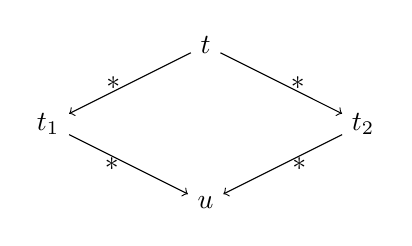
\begin{tikzpicture}	
  	\node(t) at (0,2) {$t$}; 
	\node(t1) at (-2,1) {$t_1$};
   	\node(t2) at (2,1) {$t_2$};
	\node (u) at (0,0) {$u$};
	\draw [->]  (t) --node[midway,left]{$*$} (t1) ;
	\draw [->]  (t) --node[midway,right]{$*$} (t2) ;
	\draw [->]  (t1) --node[midway,left]{$*$} (u) ;
	\draw [->]  (t2) --node[midway,right]{$*$} (u) ;
   \end{tikzpicture}
\end{figure} 
\end{block}
\end{frame}

\begin{frame}[fragile]{$\beta$-forma normal\u a}

Intuitiv, o form\u a normal\u a este  un termen care nu mai poate fi redus (sau punctul final al unui calcul). 

\begin{block}{Form\u a normal \u a}
\begin{itemize}
\item un $\lambda$-termen c\u aruia nu i se  mai poate aplica reducerea \^{\i}ntr-un pas $\ra_\beta$  se nume\sh te {\it $\beta$-form\u a normal\u a}
\item dac\u a $t\sra_\beta u_1$, $t\sra_\beta u_2$ \sh i $u_1$, $u_2$ sunt $\eta$-forme normale atunci, datorit\u a confluen\ts ei, $u_1=_\alpha u_2$
\item un $\lambda$-termen poate avea cel mult o $\beta$-form\u a normal\u a (modulo $\alpha$-echivalen\ts \u a)
\end{itemize}
\end{block}

\end{frame}

\begin{frame}[fragile]{$\beta$-forma normal\u a}

\begin{block}{Form\u a normal \u a}
\begin{itemize}
\item un $\lambda$-termen c\u aruia nu i se  mai poate aplica reducerea \^{\i}ntr-un pas $\ra_\beta$  se nume\sh te {\it $\beta$-form\u a normal\u a}
\item dac\u a $t\sra_\beta u_1$, $t\sra_\beta u_2$ \sh i $u_1$, $u_2$ sunt $\eta$-forme normale atunci, datorit\u a confluen\ts ei, $u_1=_\alpha u_2$
\item un $\lambda$-termen poate avea cel mult o $\beta$-form\u a normal\u a (modulo $\alpha$-echivalen\ts \u a)
\end{itemize}
\end{block}

Exemplu:
\begin{itemize}
\item $zv$ este $\beta$-form\u a normal\u a pentru  $(\lambda x.(\lambda y.yx)z)v$

$(\lambda x.(\lambda y.yx)z)v\ra_\beta (\lambda y.yv)z\ra_\beta zv$

\item exist\u a termeni care {\bf nu} pot fi redu\sh i la o $\beta$-form\u a normal\u a, de exemplu $(\lambda x. xx)(\lambda x. xx)$

\end{itemize}

\end{frame}


\begin{frame}[fragile]{$\beta$-conversia}

Intuitiv, $\beta$-conversia extinde $\beta$-reduc\ts ia \^{\i}n ambele direc\ts ii. 



\begin{itemize}
\item $(\lambda y. yv) z\ra_\beta zv \leftarrow_\beta (\lambda x.zx)v$\pause

\item $(\lambda y. yv) z\leftarrow_\beta (\lambda x.(\lambda y.yx)z)v \ra_\beta (\lambda x.zx)v$
\end{itemize}
\pause

\begin{block}{$\beta$-conversia  $=_\beta$}
\begin{itemize}
\item $=_\beta\subseteq \Lambda T\times \Lambda T$

$t_1=_\beta  t_2$ dac\u a  exist\u a $n\geq 0$ \sh i $u_0,\ldots, u_n$ astfel \^{\i}nc\^{a}t

$t_1=_\alpha u_0$, $u_n =_\alpha t_2$ \sh i, pentru orice $i$,
$u_i\ra_\beta u_{i+1}$ sau $u_{i+1}\ra_\beta u_{i}$

\end{itemize}
\end{block}

\pause

Exemplu: $(\lambda y. yv) z =_\beta (\lambda x.zx)v $
\end{frame}

\begin{frame}[fragile]{$\beta$-conversia}


\begin{block}{$\beta$-conversia  $=_\beta$}
\begin{itemize}
\item $=_\beta\subseteq \Lambda T\times \Lambda T$

$t_1=_\beta  t_2$ dac\u a  exist\u a $n\geq 0$ \sh i $u_0,\ldots, u_n$ astfel \^{\i}nc\^{a}t

$t_1=_\alpha u_0$, $u_n =_\alpha t_2$ \sh i, pentru orice $i$,
$u_i\ra_\beta u_{i+1}$ sau $u_{i+1}\ra_\beta u_{i}$

\end{itemize}
\end{block}\pause

\begin{block}{Observa\ts ii}
\begin{itemize}
\item $=_\beta$ este o rela\ts ie de echivalen\ts \u a\pause
\item pentru  $t_1$, $t_2$ $\lambda$-termeni \sh i $u_1$, $u_2$  $\beta$-forme normale 

dac\u a $t_1\sra_\beta u_1$, $t_2\sra_\beta u_2$ \sh i $u_1=_\alpha u_2$ atunci $t_1=_\beta t_2$
\end{itemize}
\end{block}

\end{frame}


\begin{frame}[fragile]{$\beta$-conversia}
\begin{block}{$\beta$-conversia  $=_\beta$}
\begin{itemize}
\item $=_\beta\subseteq \Lambda T\times \Lambda T$

$t_1=_\beta  t_2$ dac\u a  exist\u a $n\geq 0$ \sh i $u_0,\ldots, u_n$ astfel \^{\i}nc\^{a}t

$t_1=_\alpha u_0$, $u_n =_\alpha t_2$ \sh i, pentru orice $i$,
$u_i\ra_\beta u_{i+1}$ sau $u_{i+1}\ra_\beta u_{i}$

\item $=_\beta$ este o rela\ts ie de echivalen\ts \u a\pause
\item pentru  $t_1$, $t_2$ $\lambda$-termeni \sh i $u_1$, $u_2$  $\beta$-forme normale 

dac\u a $t_1\sra_\beta u_1$, $t_2\sra_\beta u_2$ \sh i $u_1=_\alpha u_2$ atunci $t_1=_\beta t_2$
\end{itemize}
\end{block}

\medskip

{\it $\beta$-conversia reprezint\u a "egalitatea prin calcul", iar $\beta$-reduc\ts ia (modulo $\alpha$-conversie) ofer\u a o procedur\u a de decizie pentru aceasta. }
\end{frame}

\begin{frame}{}
\vfill\begin{center}
\intens{Pe s\u apt\u am\^ana viitoare!}
\end{center}
\vfill
\end{frame}
\end{document}



